% Adapted from the organizers' official read-only Overleaf template.
\documentclass[sigconf]{acmart}
% Setup from the official competition report template.
\setcopyright{none}
\settopmatter{printacmref=false}
\acmConference[Kaggle Competition]{Filament Segmentation Challenge}{2026}{\href{https://www.kaggle.com/competitions/filament-segmentation-2026}{kaggle.com/competitions/filament-segmentation-2026}}
\acmBooktitle{Competition Report}
\acmDOI{}
\acmISBN{}
\usepackage{xcolor}
\newif\ifguideStyle
\guideStyletrue
\newcommand{\guide}[1]{\ifguideStyle{\color{gray!65}\itshape #1}\fi}
\usepackage{mathtools}
\usepackage{subcaption}
\usepackage{tabularx}
\usepackage{multirow}

\guideStylefalse
\begin{document}
\title{Instance Segmentation of Solar Filaments in GONG Observations}
\subtitle{A Solution to the Solar Filament Segmentation Challenge 2026}
\IfFileExists{author.local.tex}{\input{author.local}}{\author{James Nojek}
\affiliation{\city{Houston}\state{Texas}\country{United States}}
}
\begin{abstract}
This report describes our solution to the Solar Filament Segmentation Challenge~2026, a Kaggle competition on automatic segmentation of solar filaments in GONG H-$\alpha$ observations. We trained a compact U-Net on native-resolution image crops and reconstructed per-disk instance masks by blending overlapping tiles. On grouped development observations the model achieved pooled Panoptic Quality of 0.3365. A matched contrast filter removed unsupported detections but erased too many annotated structures under a predeclared miss limit, so we retained the baseline. We independently checked the organizer scorer and decoded the complete native-resolution export.
\end{abstract}
\maketitle

\section{Introduction}
This report goes over the details of our solution to the Solar Filament Segmentation Challenge~2026 \cite{filament-segmentation-2026}. The challenge, launched on July~10,~2026, is organized by the Earth-Space AI Research (ESAIR) Lab\footnote{\href{https://www.esairlab.com/home}{www.esairlab.com/}}. This challenge utilizes the MAGFiLO dataset for evaluation of the segmentation algorithms \cite{ahmadzadeh2024dataset}.
We build a native-pixel U-Net baseline and test a single mechanism selected from its held-out development errors. The comparison separates reproducibility, instance-level scoring and qualitative failure review. We keep the output in the supplied disk coordinates, including small and faint structures where the model has evidence for them.


\section{Methodology}\label{sec:methodology}
\subsection{Data and split}
The supplied competition data contain 707 physical training disks and 180 unlabeled test disks. Images are grayscale, 8-bit JPEGs at \(2048\times2048\) pixels. The training JSON contains 1,154 independent annotator views and 8,199 nonempty filament annotations. Multiple views of a JPEG share one physical image ID; an annotator prefix identifies the view. We decode each polygon into a native binary mask with COCO utilities. We use no external labels, observations, weights or inference inputs.

We place physical images in 27-day UTC blocks and reserve Udaipur as the site transfer test. A 48-hour temporal embargo removes cross-fold neighbors. The final split contains 336 training, 115 development, 80 confirmation, 101 site-transfer and 75 purged disks. The closest retained cross-fold pair is 48 hours and 20 seconds apart. An independent audit found no repeated JPEG bytes or high-correlation pairs in a low-resolution image screen. This reduces the risk of nearly repeated images crossing the split; it does not prove that long-lived features never recur.

\subsection{Image representation and model}
For each disk, we sample pixels from the central square and subtract its median. We divide by the 90th-to-10th percentile range with a 16-gray-level floor and clip to \([-4,4]\). This retains local dark contrast while limiting the effect of exposure differences. Development annotations show median skeleton width of approximately 8.3 native pixels, so we retain native pixels in the network and export.

Our compact U-Net \cite{ronneberger2015unet} uses five encoder levels, four decoder stages, two \(3\times3\) convolutions per block, group normalization and SiLU activations. Base width is 24 and doubles on each downsampling step; the model has 4.37 million parameters. Transposed convolutions upsample the decoder, which receives encoder features at each scale through skip connections. The final \(1\times1\) convolution predicts a foreground logit.

For each annotation view we take the union of its filament masks. The mean of these unions across views gives a soft training label, so ambiguous pixels need not be forced to a binary consensus. We sample five \(384\times384\) crops per physical observation per epoch. With probability 0.65 we anchor a crop near an annotated bounding box, with bounded jitter; otherwise we sample uniformly. We apply right-angle rotations, a random reflection and modest intensity scaling and shifts. The training objective is pixel-weighted binary cross entropy plus soft Dice loss. AdamW starts at \(7\times10^{-4}\) and uses a cosine schedule. We train from random initialization, with batch size 12 and seed 271828, on an RTX 4090.

\subsection{Native inference and instance extraction}
We tile the normalized \(2048\times2048\) disk at stride 288 with the last tile aligned to each edge. We accumulate sigmoid probabilities with taper weights near overlap boundaries and divide by the total weight at each pixel. The reconstructed probability map is stored as float16 before instance extraction. An independent pointwise fixture checked every reconstructed pixel and found a maximum error of \(2.44\times10^{-4}\) after float16 rounding. This checks tile placement; a four-disk development check reproduced the chosen stride exactly but changing it to 256 shifted foreground IoU to 0.876--0.922. We therefore lock the tiling grid for reproduction.

We threshold the native map, use eight-neighbor connected components and drop regions smaller than a calibrated area. A fixed 24-image development subset selects epoch 24. We then recalibrate on all 115 development maps and freeze a probability threshold of 0.65 and minimum area of 700 native pixels. Confirmation and site-transfer observations play no role in either decision. Each output instance is one native compressed COCO RLE. Its row ID combines the unchanged observation stem and a unique suffix. For images with zero predicted instances, the export emits no placeholder row, and the coverage record still accounts for the image.

\begin{figure*}[t]
\centering
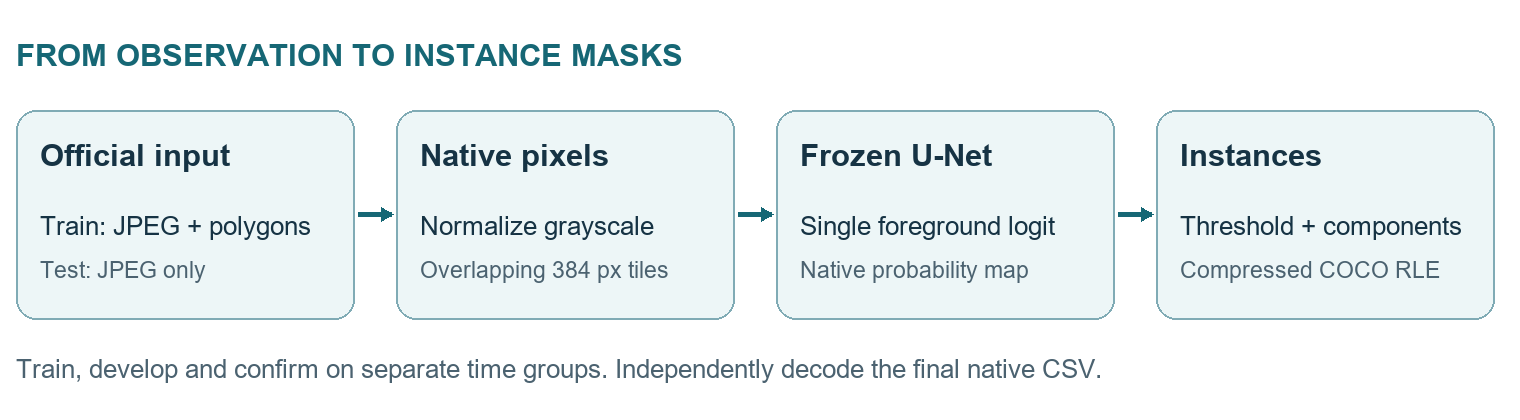
\includegraphics[width=\textwidth]{pipeline.png}
\caption{Training and inference paths. Test inference uses the supplied H-\(\alpha\) JPEG and the frozen model.}
\end{figure*}

\subsection{Challenger: disk-aware local contrast}
We considered short-gap repair because GONG seeing and opacity variation can interrupt an otherwise coherent filament. The development audit found 298 predictions with zero overlap with the corresponding annotation view: 101 in the disk interior, 189 at projected radius \(0.8\) to \(0.95\,R\), two near the rim and six off disk. It found 73 meaningful splits but only six with a short, directionally supported gap. Only one of those had a fragment pair whose truth-informed union would recover a missed match. We therefore tested local contrast as the single challenger.

For each disk we fit a circle to outward intensity drops along 180 radial rays. For each baseline instance we skeletonize the component, estimate width from its interior distance transform and sample an adjacent flank band. Flank pixels must lie within \(0.98\,R\) and outside any predicted foreground. With flank median \(m_f\), skeleton median \(m_s\) and flank median absolute deviation \(d_f\), the score is
\[
 c=\frac{m_f-m_s}{\max(2,\ 1.4826d_f)}.
\]
A component is retained unchanged if its score meets the contrast floor. We retain the baseline instance when the disk fit or local background is unreliable. The challenger changes neither network probabilities nor accepted mask boundaries. The floor is selected on development groups, keeping all other settings and inputs fixed.

H-\(\alpha\) contrast is an observed intensity difference, not evidence of magnetic connectivity. Dark active-region structures can pass the filter, and genuine faint structures can fail it. GONG display JPEGs already suppress large-scale intensity variation; we use local flanks rather than fitting a global limb-darkening correction.



\section{Evaluation}\label{sec:evaluation}
\subsection{Metric and diagnostics}
We follow the organizer's published self-evaluation notebook. Every prediction set is compared separately with each annotator view of the same physical disk. A match requires instance IoU strictly above 0.5. We sum matched IoUs and pool counts over annotator views:
\[
 \mathrm{PQ}=\frac{\sum_{(p,t)\in\mathrm{TP}}\operatorname{IoU}(p,t)}
 {|\mathrm{TP}|+0.5|\mathrm{FP}|+0.5|\mathrm{FN}|}.
\]
This is the organizer's implementation of the PQ approach \cite{kirillov2019panoptic}. Independent full-resolution fixtures verified perfect masks, misses, splits, merges, the strict threshold, and the notebook treatment of images with no predictions. We distinguish the organizer's any-overlap split and merge counts from diagnostic counts that require substantial overlap.

Thin and faint cutoffs are fixed from development annotations before confirmation. Thin means median skeleton width at most 6.32 pixels. Faint means a local flank-normalized contrast at most 2.02. Near limb means median projected spine radius at least 0.8 times the fitted apparent disk radius. Those slices overlap. The annotation procedure omits some small, faint and near-limb cases, so conclusions apply to the available annotations.

\subsection{Matched results and selection}

\begin{table}[h]\centering\small

\caption{Matched instance scoring. Each result is pooled over independent views.}

\begin{tabular}{llrrr}

\toprule

Partition & Method & PQ & FP & FN\\

\midrule

Development & Baseline & 0.3365 & 655 & 699\\

Development & Contrast & 0.3466 & 524 & 719\\

Confirmation & Baseline & 0.2931 & 472 & 480\\

Confirmation & Contrast & 0.2978 & 405 & 492\\

Udaipur & Baseline & 0.3385 & 584 & 512\\

Udaipur & Contrast & 0.3500 & 476 & 525\\

\bottomrule

\end{tabular}

\end{table}

\begin{table}[h]\centering\small

\caption{Diagnostic errors for baseline \(\rightarrow\) contrast.}

\begin{tabular}{lrrrr}

\toprule

Partition & Splits & Merges & Zero overlap & New misses\\

\midrule

Development & 73\(\to\)67 & 12\(\to\)11 & 298\(\to\)189 & 37\\

Confirmation & 87\(\to\)79 & 5\(\to\)5 & 177\(\to\)126 & 16\\

Udaipur & 70\(\to\)61 & 6\(\to\)6 & 274\(\to\)188 & 27\\

\bottomrule

\end{tabular}

\end{table}

Development: 115 disks, 186 views, 1375 annotated instances; PQ change +0.0101; paired 95\% bootstrap interval [+0.0060, +0.0148].

Confirmation: 80 disks, 127 views, 846 annotated instances; PQ change +0.0047; paired 95\% bootstrap interval [-0.0045, +0.0117].

Udaipur: 101 disks, 165 views, 1065 annotated instances; PQ change +0.0115; paired 95\% bootstrap interval [+0.0064, +0.0170].

\par\smallskip

The baseline was selected before opening confirmation. The least aggressive contrast floor, 1.8, raised development PQ but created 37 complete misses, exceeding the predeclared cap of seven. We carried this rejected setting into confirmation and the site holdout as a fixed diagnostic. Removing a component can reduce split counts without connecting a filament; this challenger never adds pixels.

\subsection{Thin, faint and near-limb instances}

\begin{table}[h]\centering\small

\caption{Confirmation match recall at instance IoU \(>0.5\).}

\begin{tabular}{lrrr}

\toprule

Slice & Truth masks & Baseline & Contrast\\

\midrule

Thin & 209 & 27.3\% & 26.8\%\\

Faint & 221 & 22.2\% & 18.1\%\\

Near limb & 107 & 57.0\% & 50.5\%\\

\bottomrule

\end{tabular}

\end{table}

On confirmation, the 0.0047 PQ gain fell below the predeclared 0.005 threshold, with 16 new complete misses against a cap of five. The contrast filter removes weak foreground responses, including examples with no annotation overlap, but it also removes genuine faint spines. The selected baseline preserves those detections (Fig.~2). Its remaining errors include isolated dark structures, disconnected portions of annotated filaments and under-coverage of faint structures. Some cases are ambiguous across annotators. Neither the foreground model nor the filter establishes physical connectivity.

The host identified PQ above 0.35 as scientifically useful in its August 20 announcement. That figure is a reference point rather than a finalist threshold. Reche and Cid \cite{reche2026} report held-out MAGFiLO crop IoU 0.70 and Dice 0.81 using a U-Net trained on MAGFiLO and SWEFil. Their crop results have different training inputs and evaluate mask overlap with a localized target. The numbers do not translate to full-disk instance PQ. Diercke et al.\ \cite{diercke2024} document seeing-related fragmentation and confusion from other dark solar structures, motivating the split and false-positive diagnostics reported here.


\subsection{Inference and reproducibility}

The selected export processed 180 supplied test images in 76.05 seconds on the RTX 4090, with 1.15 GiB peak process RAM and 1.11 GiB peak reserved GPU memory. It contains 1,293 predicted instances and 3 disks with no emitted rows. The 324,704-byte CSV fits the 10 MB form limit. The released notebook independently decodes the exact output and checks its SHA-256.

In an independent clean process, the notebook regenerated identical CSV and coverage hashes and independently decoded every mask. The validation scores above are local. No Kaggle score was available when this report was prepared.


\IfFileExists{figures-local/examples.png}{%
\begin{figure*}[t]
\centering
\includegraphics[width=\textwidth]{figures-local/examples.png}
\caption{Representative confirmation crops. The three panes show grayscale H-\(\alpha\), the selected baseline, and the rejected contrast filter. Cyan outlines show one annotator view; amber outlines show predicted masks. Contrast filtering removes one unsupported response (B) but discards a valid near-limb match (C). The examples also show a retained match (A) and a miss by both methods (D).}
\end{figure*}
}{}


\section{Acknowledgment}\label{sec:acknowledgment}
The organization of the Filament Segmentation Challenge 2026 is partially supported by the U.S. National Science Foundation (NSF) under Grant No. 2209912 and 2433781, directorate for Computer and Information Science and Engineering (CSE), and Office of Advanced Cyberinfrastructure (OAC), and Grant No. 2511630, AST Division Of Astronomical Sciences and MPS Directorate for Mathematical and Physical Sciences.

The Filament Segmentation Challenge 2026 is sponsored by the U.S. National Science Foundation (NSF) National Solar Observatory (NSO).

This work utilizes GONG data obtained by the NSO Integrated Synoptic Program, managed by the National Solar Observatory, which is operated by the Association of Universities for Research in Astronomy (AURA), Inc. under a cooperative agreement with the National Science Foundation and with contribution from the National Oceanic and Atmospheric Administration. The GONG network of instruments is hosted by the Big Bear Solar Observatory, High Altitude Observatory, Learmonth Solar Observatory, Udaipur Solar Observatory, Instituto de Astrofísica de Canarias, and Cerro Tololo Interamerican Observatory.

\bibliographystyle{ACM-Reference-Format}
\bibliography{main}
\end{document}
